% The CSM notation legend — global/local session-type syntax, typeset.
% Palette: send=emerald, recv=sky, choice=indigo, call/box=violet, projection=teal.
\documentclass[border=10pt]{standalone}
\usepackage{tikz}
\usepackage{amssymb}
\usepackage{xcolor}
\usetikzlibrary{matrix, positioning}
\definecolor{send}{HTML}{059669}
\definecolor{recv}{HTML}{0284C7}
\definecolor{ch}{HTML}{4F46E5}
\definecolor{call}{HTML}{7C3AED}
\definecolor{proj}{HTML}{0D9488}
\definecolor{ink}{HTML}{1E293B}
\begin{document}
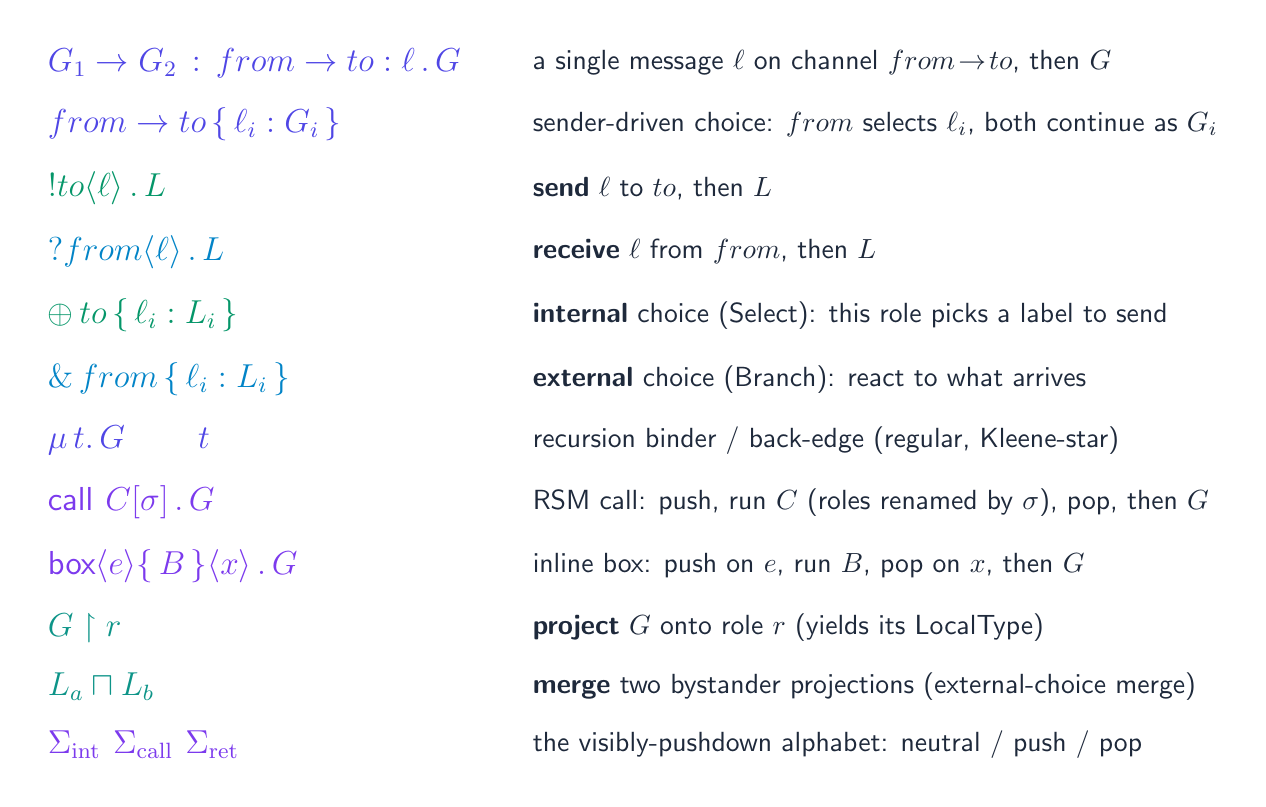
\begin{tikzpicture}[font=\sffamily]
  \matrix (m) [matrix of nodes, nodes={anchor=west, inner sep=4pt, text=ink},
    column 1/.style={nodes={font=\sffamily\bfseries\large}},
    row sep=3pt, column sep=18pt] {
    |[text=ch]| $G_{1} \to G_{2}\,:\,from \to to : \ell\,.\,G$ & a single message $\ell$ on channel $from\!\to\!to$, then $G$ \\
    |[text=ch]| $from \to to\,\{\,\ell_i : G_i\,\}$ & sender-driven choice: $from$ selects $\ell_i$, both continue as $G_i$ \\
    |[text=send]| $!to\langle \ell \rangle\,.\,L$ & \textbf{send} $\ell$ to $to$, then $L$ \\
    |[text=recv]| $?from\langle \ell \rangle\,.\,L$ & \textbf{receive} $\ell$ from $from$, then $L$ \\
    |[text=send]| $\oplus\, to\,\{\,\ell_i : L_i\,\}$ & \textbf{internal} choice (Select): this role picks a label to send \\
    |[text=recv]| $\&\, from\,\{\,\ell_i : L_i\,\}$ & \textbf{external} choice (Branch): react to what arrives \\
    |[text=ch]| $\mu\, t.\,G \qquad t$ & recursion binder / back-edge (regular, Kleene-star) \\
    |[text=call]| $\mathsf{call}\ C[\sigma]\,.\,G$ & RSM call: push, run $C$ (roles renamed by $\sigma$), pop, then $G$ \\
    |[text=call]| $\mathsf{box}\langle e\rangle\{\,B\,\}\langle x\rangle\,.\,G$ & inline box: push on $e$, run $B$, pop on $x$, then $G$ \\
    |[text=proj]| $G \restriction r$ & \textbf{project} $G$ onto role $r$ (yields its LocalType) \\
    |[text=proj]| $L_a \sqcap L_b$ & \textbf{merge} two bystander projections (external-choice merge) \\
    |[text=call]| $\Sigma_{\mathrm{int}}\ \Sigma_{\mathrm{call}}\ \Sigma_{\mathrm{ret}}$ & the visibly-pushdown alphabet: neutral / push / pop \\
  };
\end{tikzpicture}
\end{document}
